\documentclass[letterpaper,twoside]{article}

\usepackage{caption}

\usepackage[authoryear]{natbib}
\usepackage{times}
\usepackage{amsmath,amsfonts}
\usepackage{graphicx}
\usepackage{indentfirst}
\usepackage{color}
\usepackage{url}
\usepackage[paper=letterpaper]{geometry}
\usepackage{fontspec}
\setmainfont[Mapping=text-tex]{Calibri}

% revise margins
\setlength{\headheight}{0.25in}
\setlength{\headsep}{-0.25in}
\setlength{\topmargin}{0.0in}
\setlength{\textheight}{9in}
\setlength{\footskip}{0.5in}
\setlength{\oddsidemargin}{-0.25in}
\setlength{\evensidemargin}{-0.25in}
\setlength{\textwidth}{7.0in}
\setlength{\rightskip}{0pt plus 1fil} % makes ragged right

% headings
\usepackage{fancyhdr}
\pagestyle{fancy}
\fancyfoot{}
\fancyfoot[C]{K. W. Broman \emph{et al.}}
\fancyfoot[RO, LE]{\textbf{\thepage\ SI}}
\fancyhead{}
\renewcommand{\headrulewidth}{0pt}
\renewcommand{\footrulewidth}{0pt}

\captionsetup[figure]{labelsep=quad}
\captionsetup[table]{labelsep=quad}

% make figures S1, S2, ...
\renewcommand{\thefigure}{\textbf{S\arabic{figure}}}
\renewcommand{\figurename}{\textbf{Figure}}

% make tables S1, S2, ...
\renewcommand{\thetable}{\textbf{S\arabic{table}}}
\renewcommand{\tablename}{\textbf{Table}}

\begin{document}

\vspace*{8mm}
\begin{center}

\textbf{\Large Identification and correction of sample mix-ups \\[14pt]
in expression genetic data: A case study}


\bigskip \bigskip \bigskip \bigskip

\textbf{\Large SUPPLEMENT}

\bigskip \bigskip
\bigskip \bigskip


{\large Karl W. Broman$^*$,
Mark P. Keller$^{\dagger}$,
Aimee Teo Broman$^{*}$, \\[8pt]
Christina Kendziorski$^{*}$,
Brian S Yandell$^{\ddagger, \S}$,
\'Saunak Sen$^{**}$,
Alan D. Attie$^{\dagger}$}

\bigskip \bigskip

$^{*}$Department of Biostatistics and Medical Informatics,
$^{\dagger}$Department of Biochemistry,
$^{\ddagger}$Department of Statistics,
and $^{\S}$Department of Horticulture,
University of Wisconsin--Madison, Madison, Wisconsin
53706, and
$^{**}$Department of Epidemiology and Biostatistics, University
of California, San Francisco, California 94107
\end{center}




\clearpage

\begin{figure}[p]
\centerline{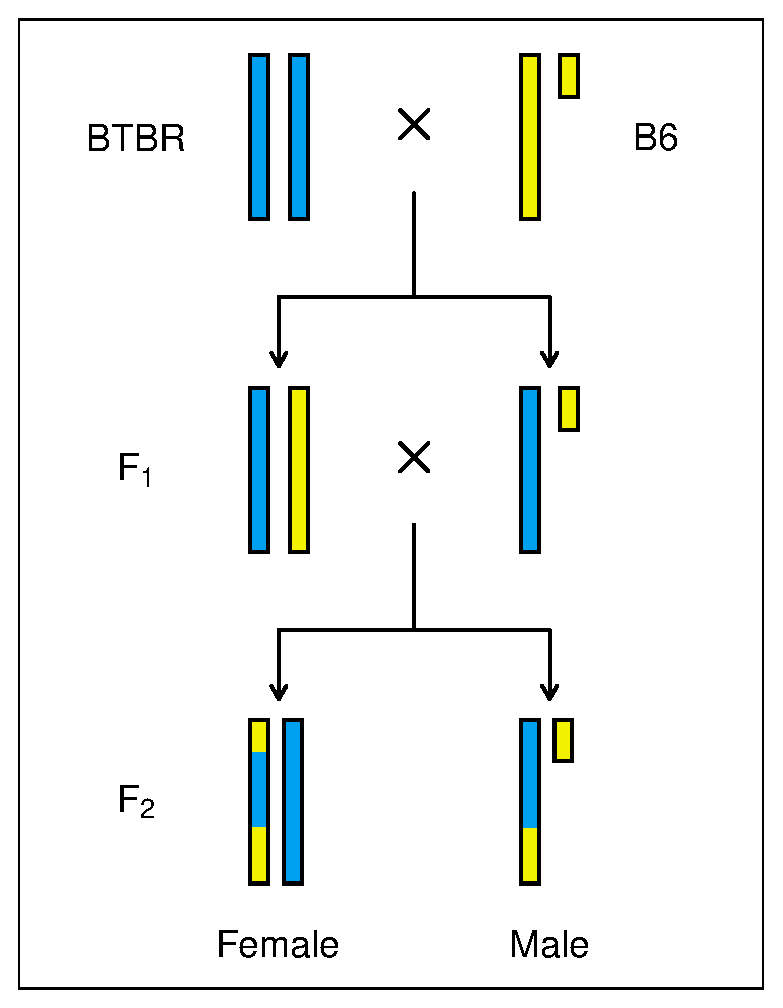
\includegraphics{SuppFigs/figS1.eps}}

\caption{KWB_FIGS1_LEGEND}
\end{figure}

\clearpage






\begin{figure}[p]
\centerline{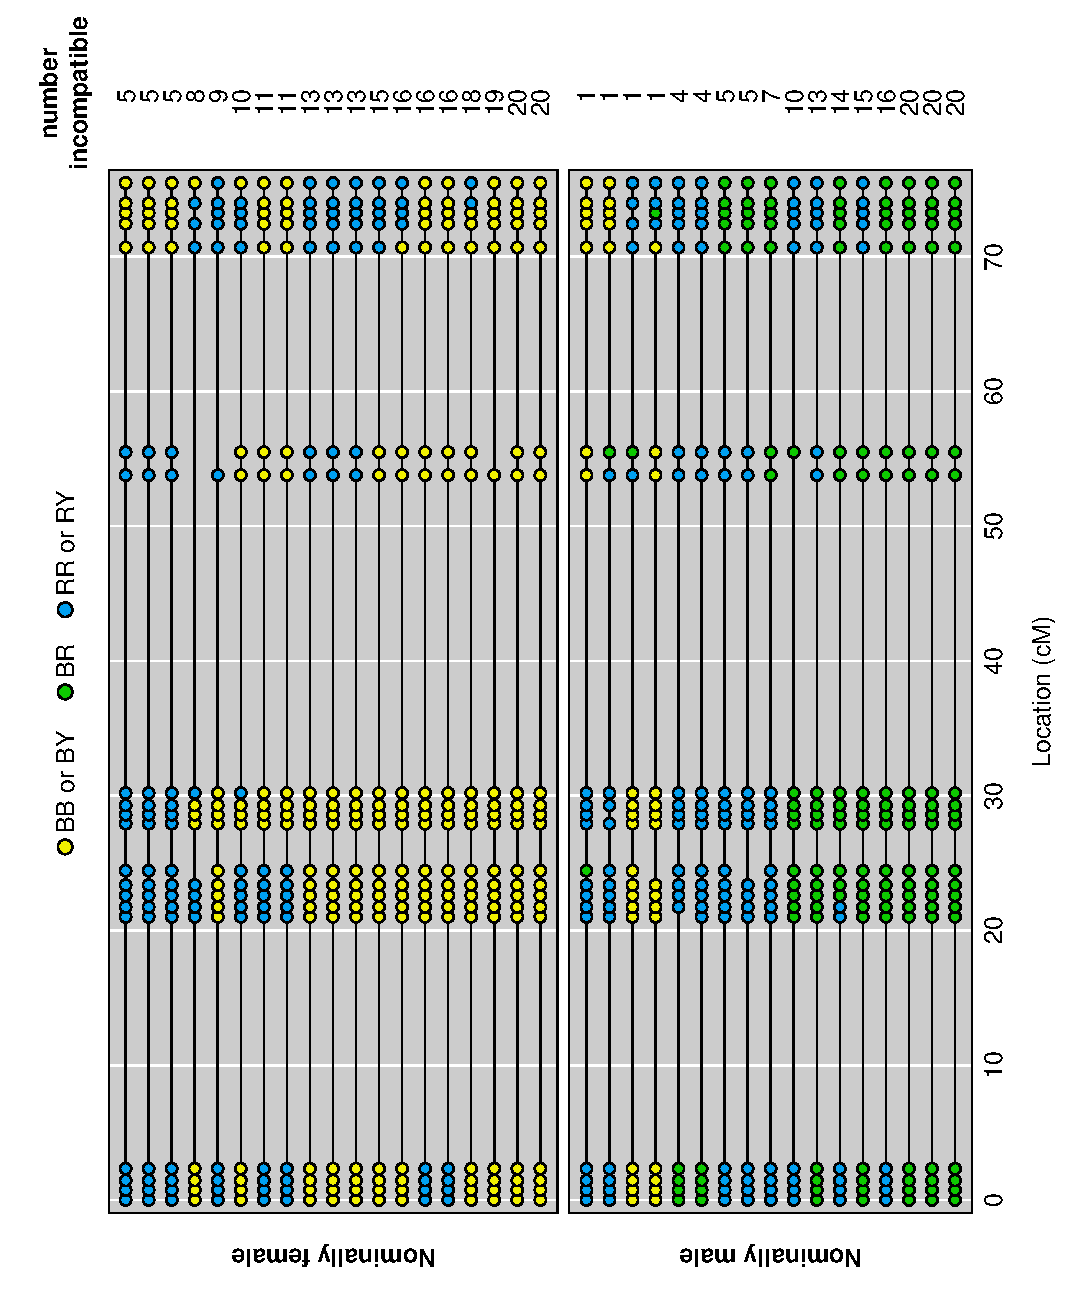
\includegraphics[angle=270,width=\textwidth]{SuppFigs/figS2.eps}}

\caption{KWB_FIGS2_LEGEND}
\end{figure}

\clearpage



\begin{figure}[p]
\centerline{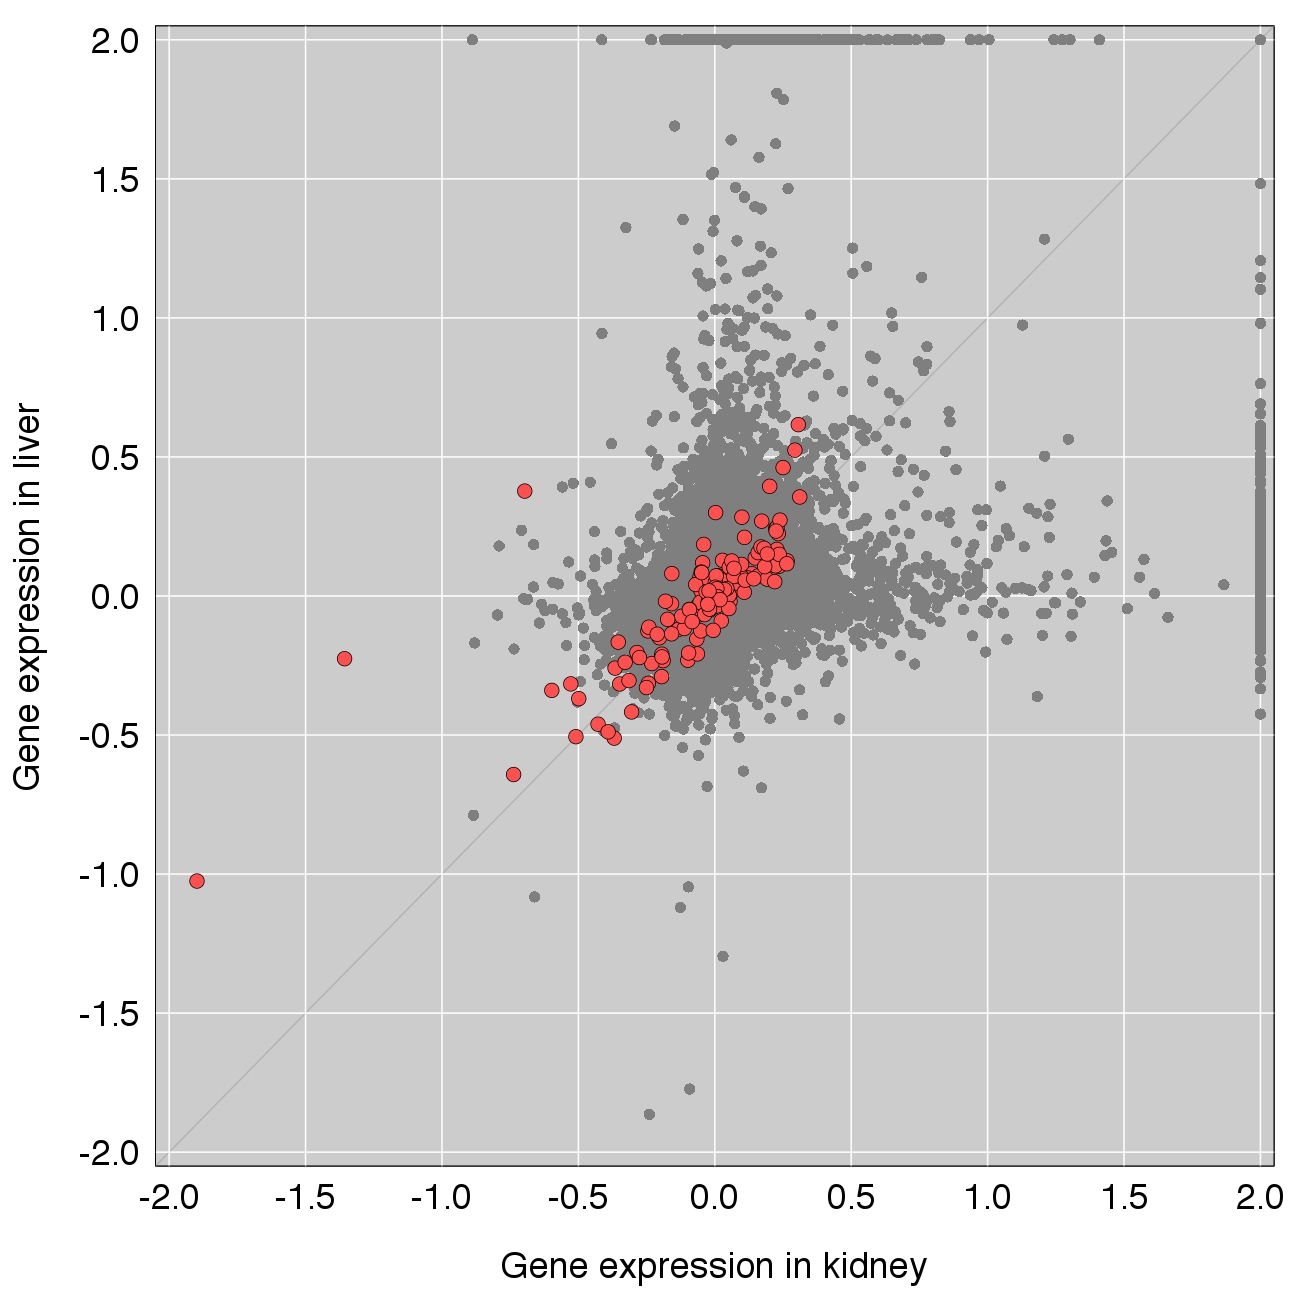
\includegraphics[width=4.5in]{SuppFigs/figS3.jpg}}

\caption{KWB_FIGS3_LEGEND}
\end{figure}


\clearpage


\begin{figure}[p]
\centerline{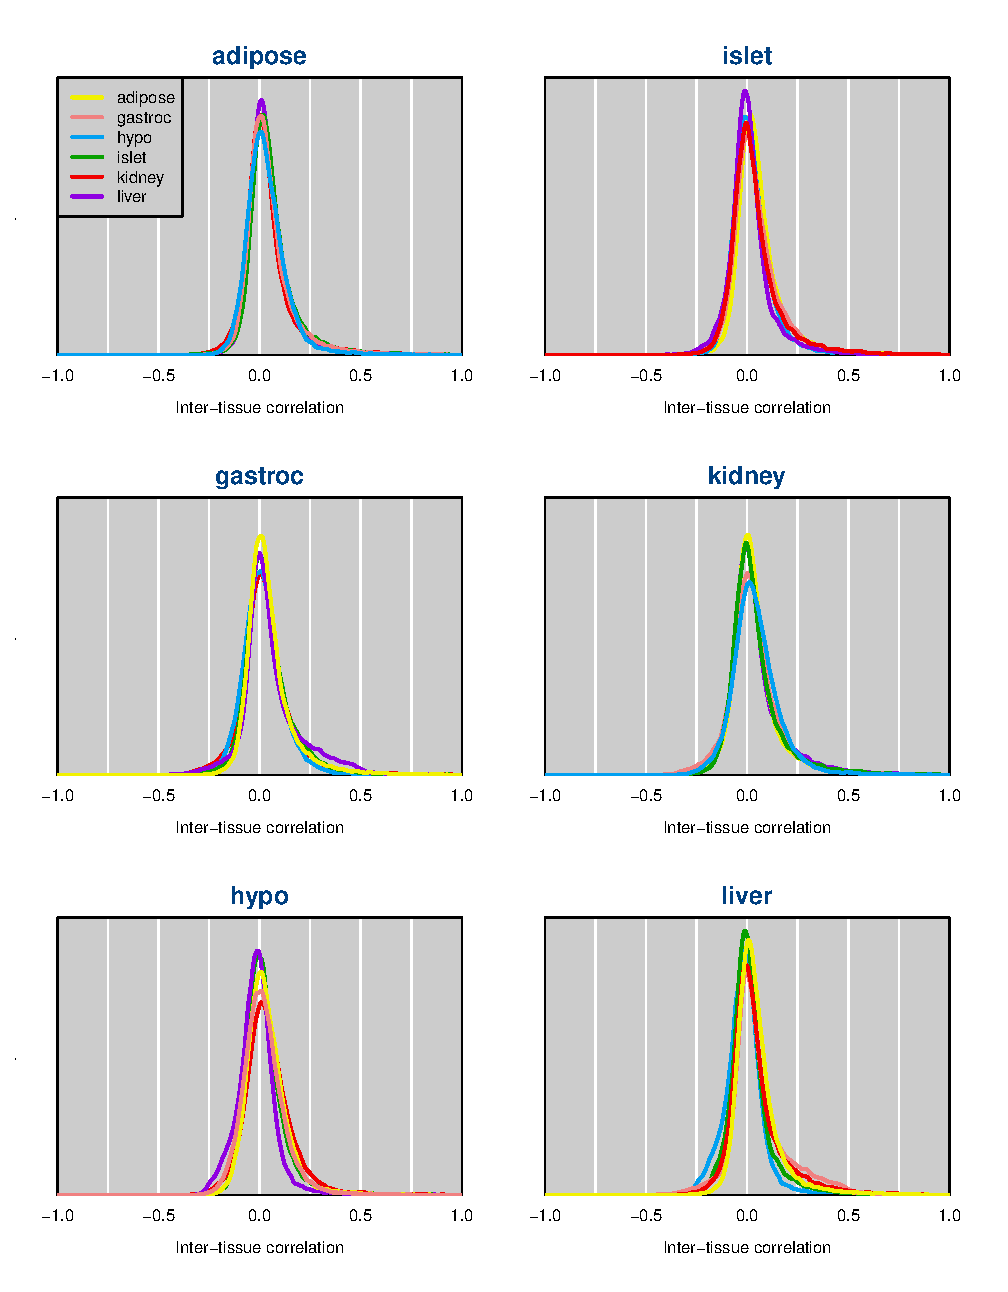
\includegraphics{SuppFigs/figS4.eps}}

\caption{KWB_FIGS4_LEGEND}
\end{figure}



\clearpage


\begin{figure}[p]
\centerline{
\includegraphics{SuppFigs/figS5.eps}}

\caption{KWB_FIGS5_LEGEND}
\end{figure}



\clearpage



\begin{figure}[p]
\centerline{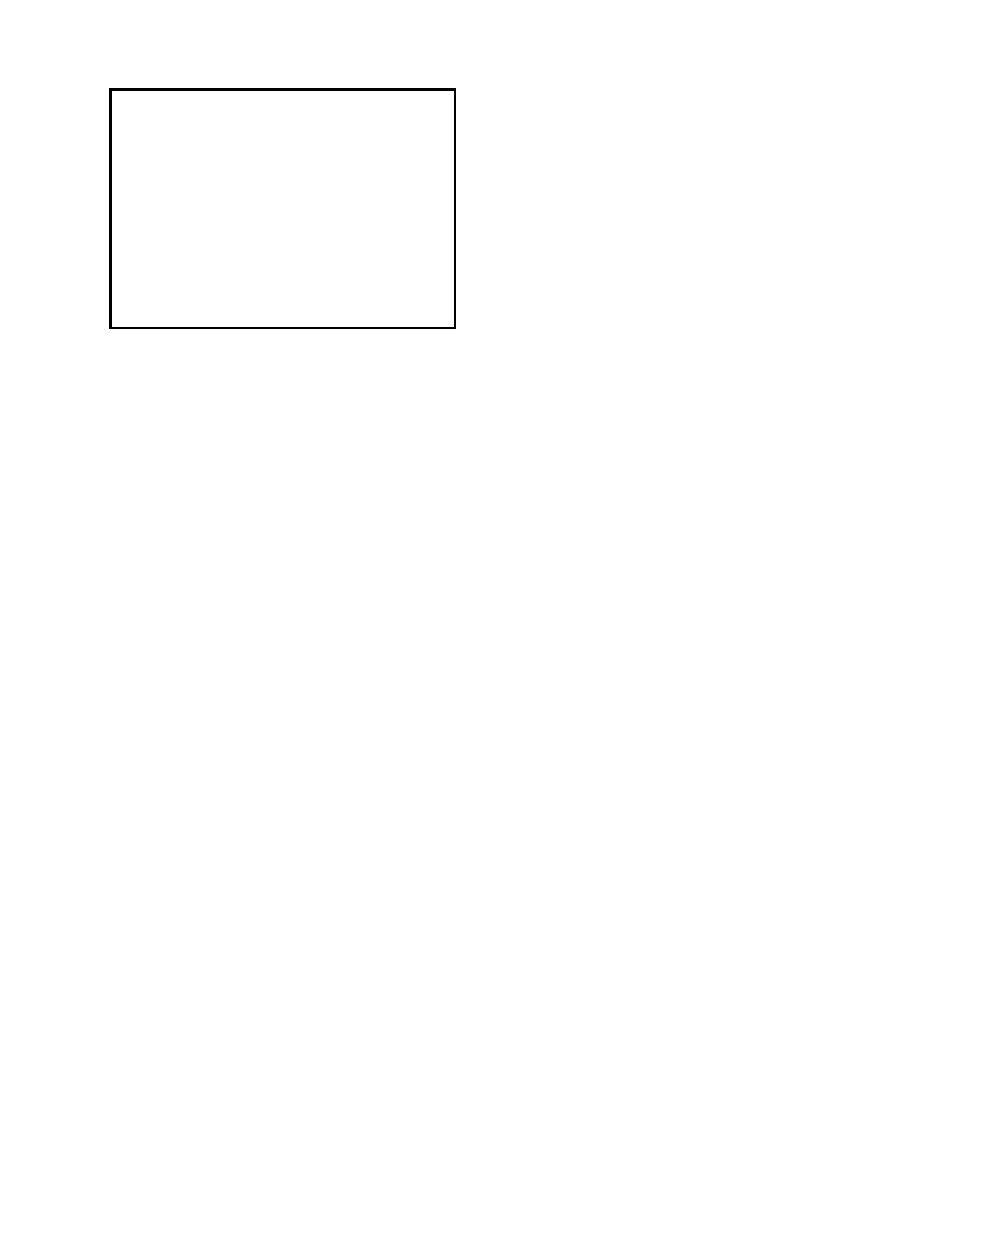
\includegraphics{SuppFigs/figS6.eps}}

\caption{KWB_FIGS6_LEGEND}
\end{figure}


\clearpage



\begin{figure}[p]
\centerline{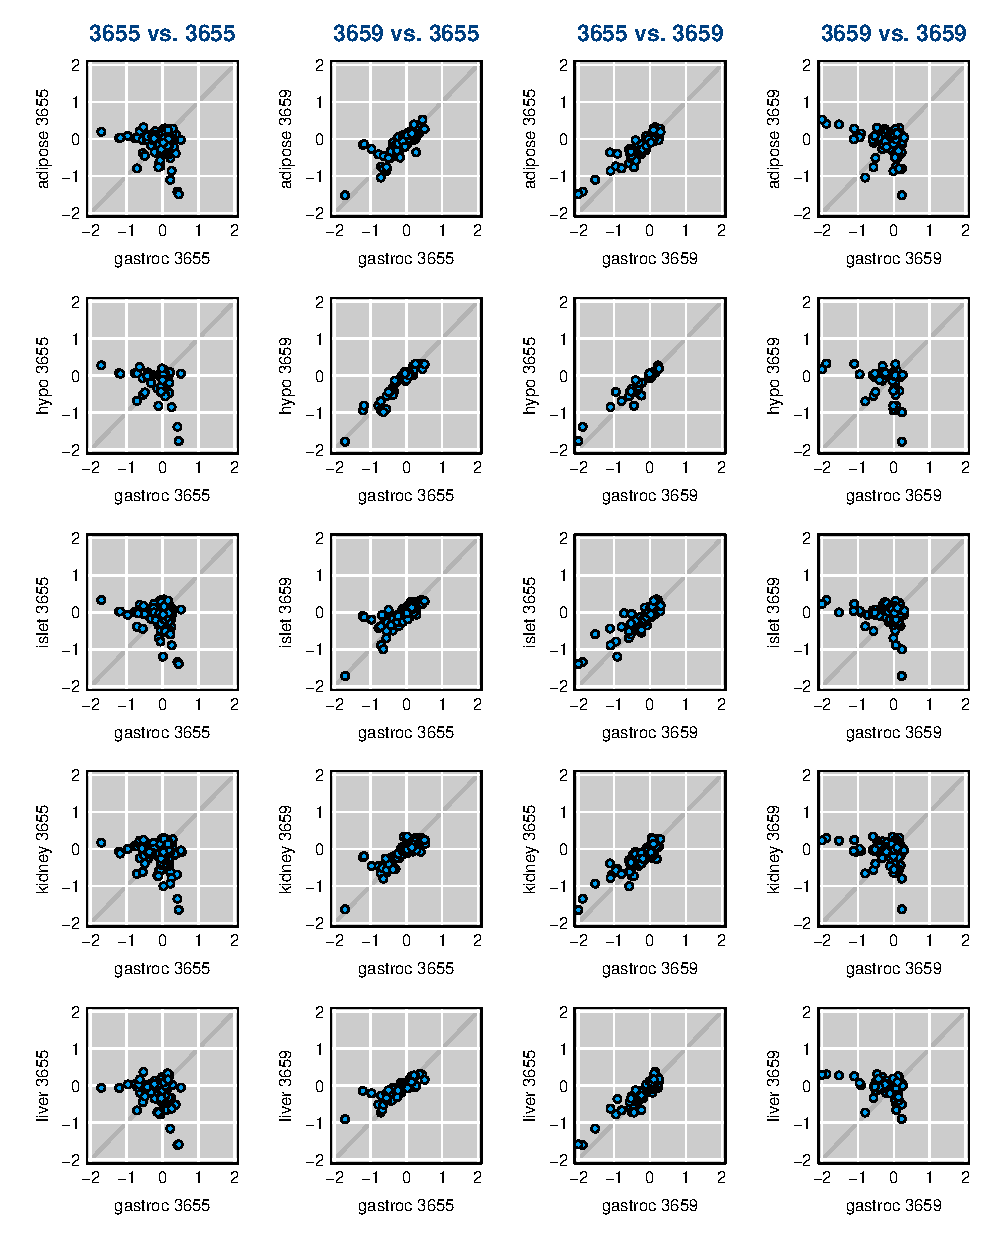
\includegraphics{SuppFigs/figS7.eps}}

\caption{KWB_FIGS7_LEGEND}
\end{figure}


\clearpage



\begin{figure}[p]
\centerline{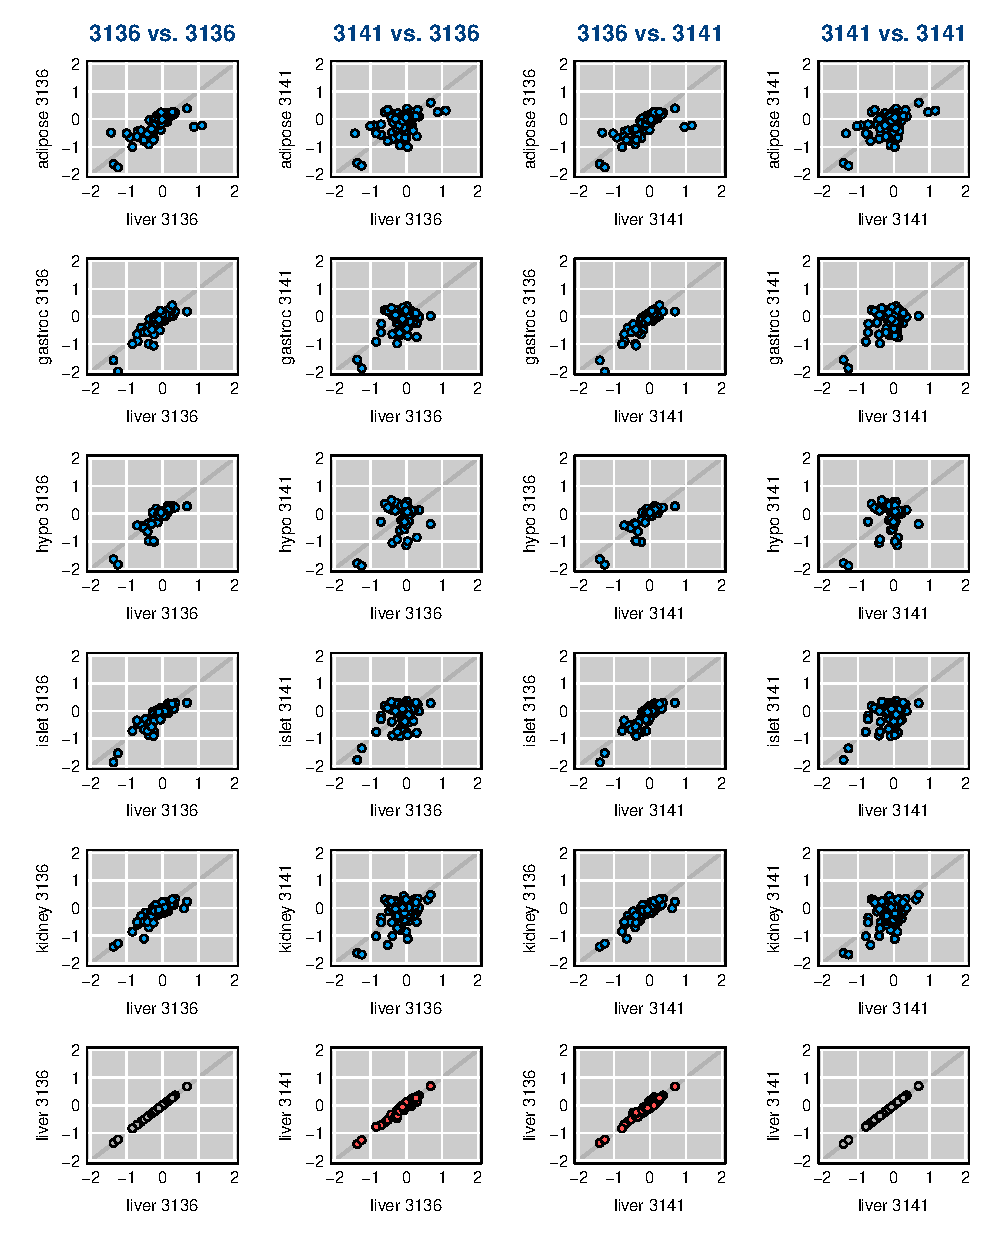
\includegraphics{SuppFigs/figS8.eps}}

\caption{KWB_FIGS8_LEGEND}
\end{figure}


\clearpage



\begin{figure}[p]
\centerline{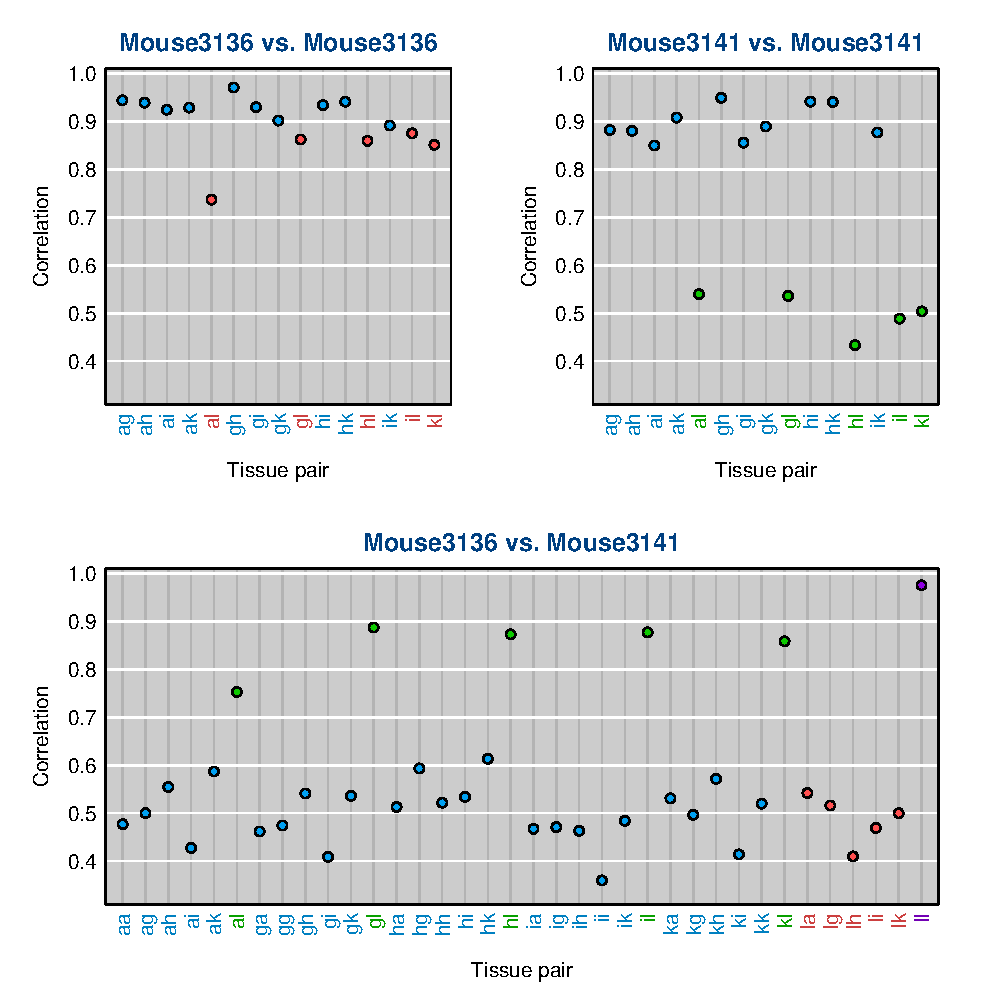
\includegraphics{SuppFigs/figS9.eps}}

\caption{KWB_FIGS9_LEGEND}
\end{figure}


\clearpage



\begin{figure}[p]
\centerline{
\includegraphics{SuppFigs/figS10.eps}}

\caption{KWB_FIGS10_LEGEND}
\end{figure}


\clearpage



\begin{figure}[p]
\centerline{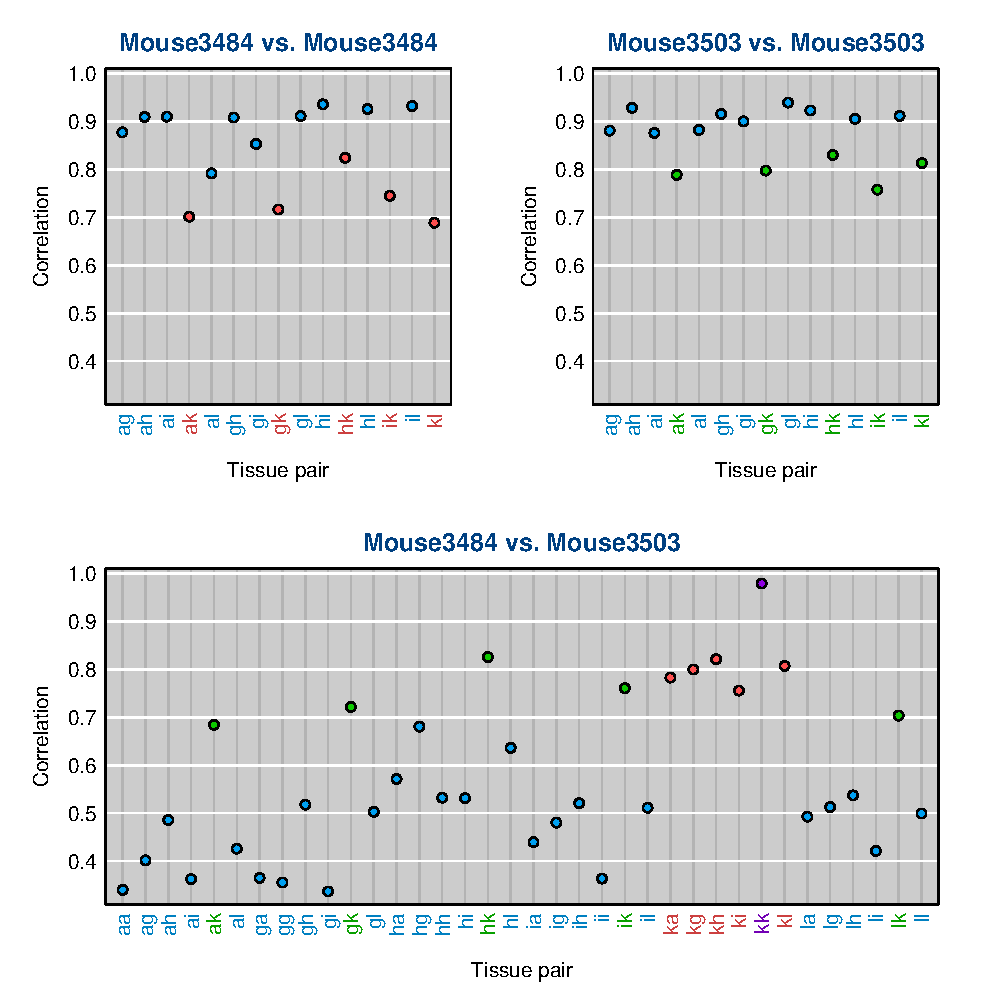
\includegraphics{SuppFigs/figS11.eps}}

\caption{KWB_FIGS11_LEGEND}
\end{figure}


\clearpage




\begin{figure}[p]
\centerline{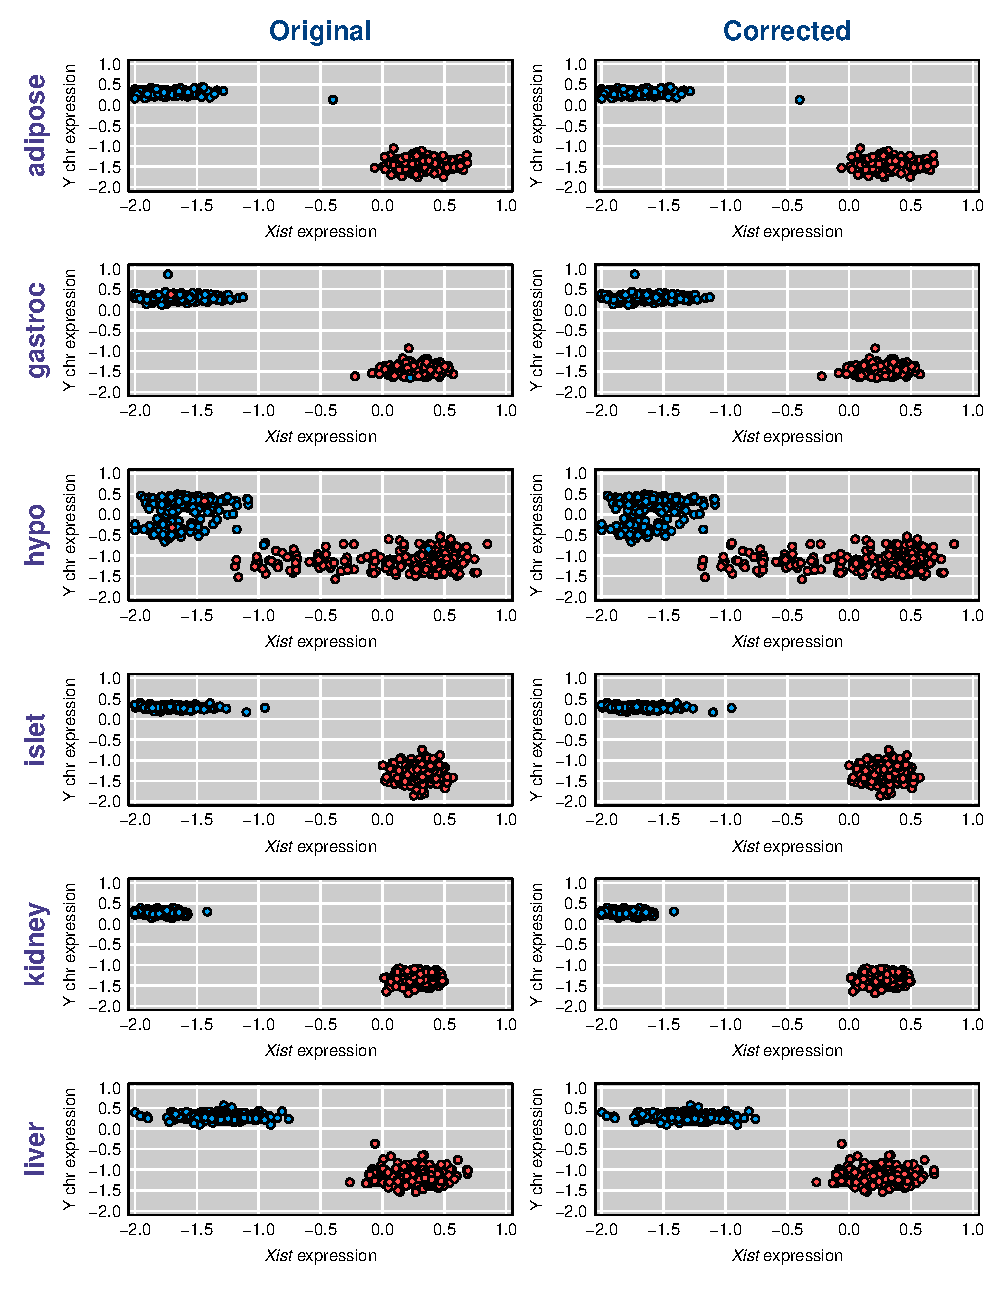
\includegraphics[height=8.0in]{SuppFigs/figS12.eps}}

\caption{KWB_FIGS12_LEGEND}
\end{figure}



\clearpage



\begin{figure}[p]
\centerline{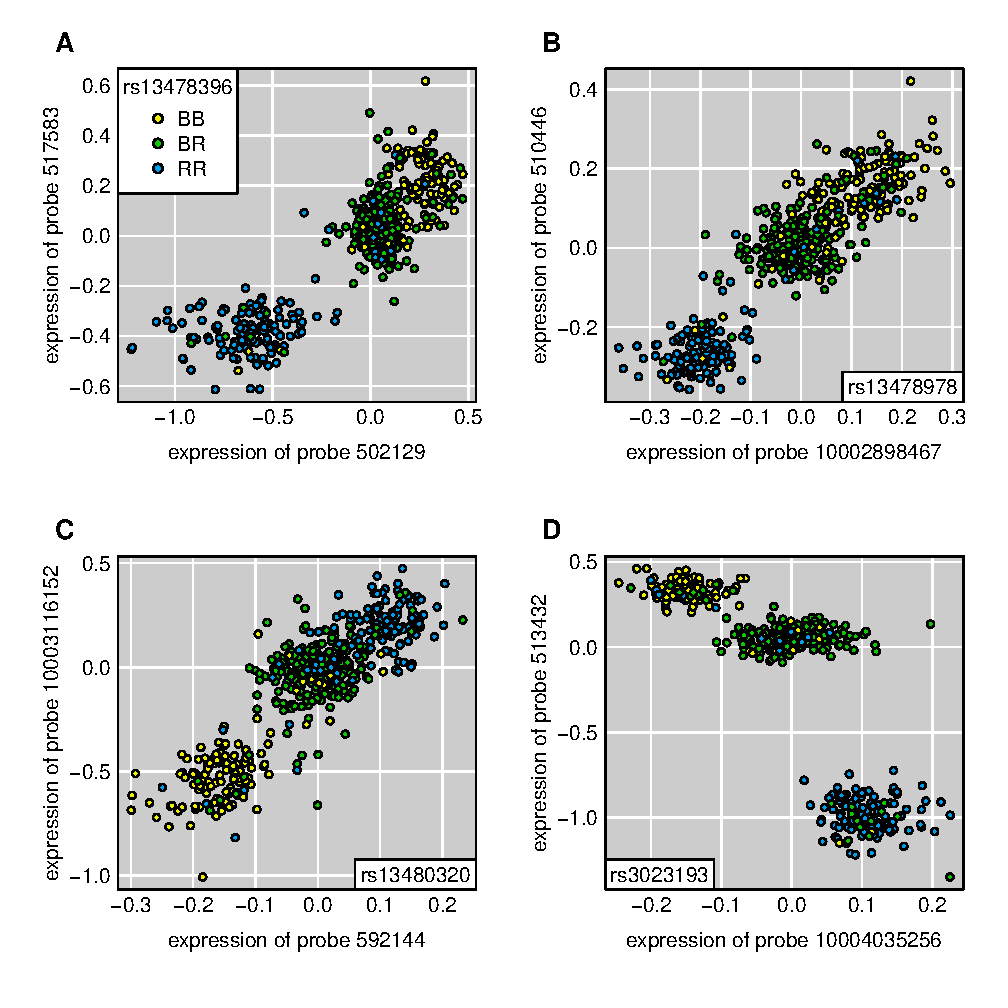
\includegraphics{SuppFigs/figS13.eps}}

\caption{KWB_FIGS13_LEGEND}
\end{figure}


\clearpage



\begin{figure}[p]
\centerline{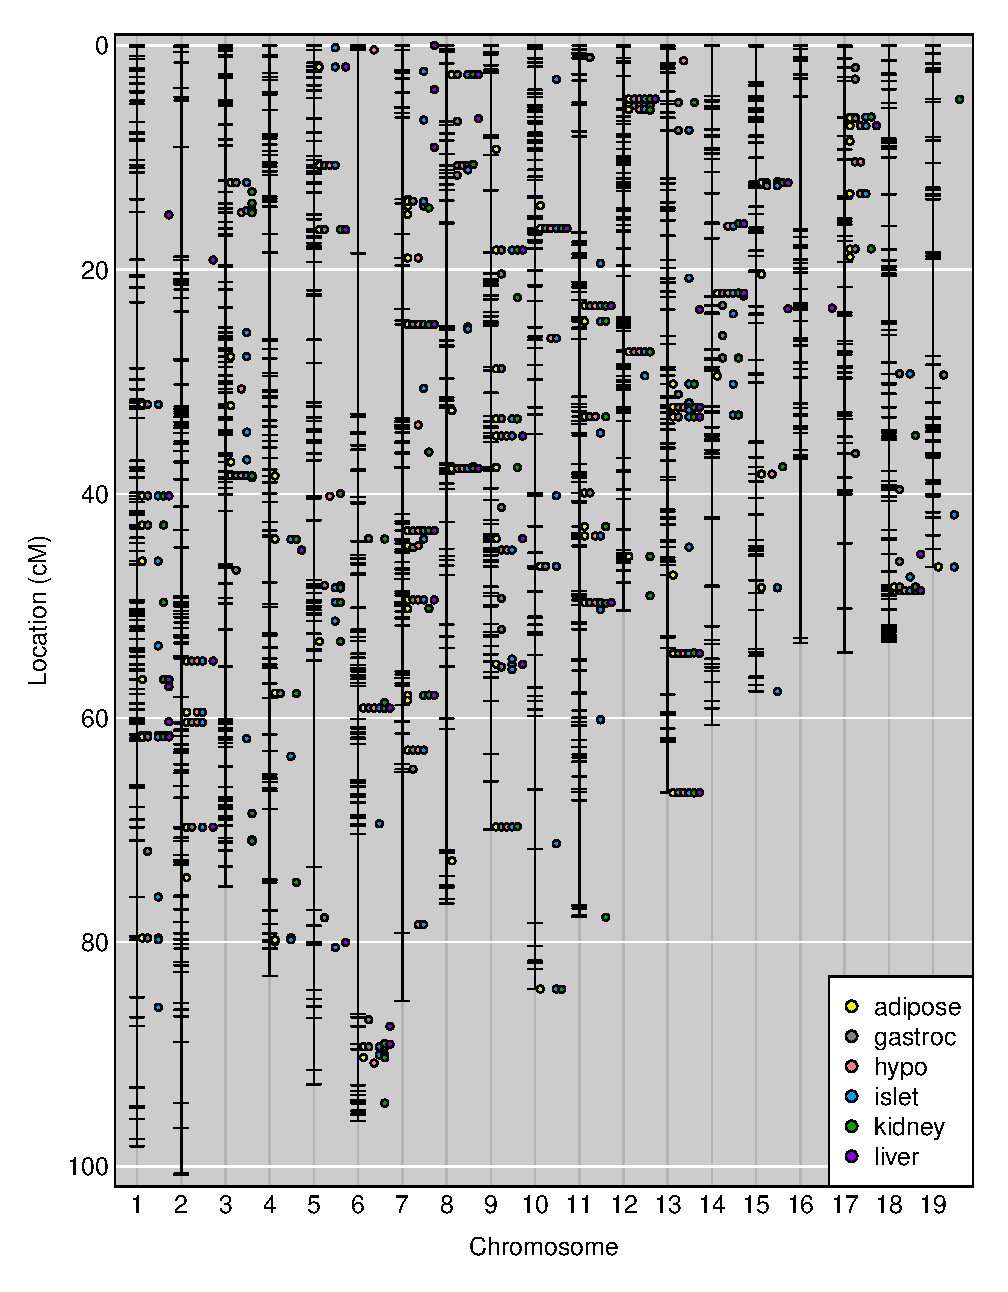
\includegraphics[height=8.0in]{SuppFigs/figS14.eps}}

\caption{KWB_FIGS14_LEGEND}
\end{figure}




\clearpage


\begin{figure}[p]
\centerline{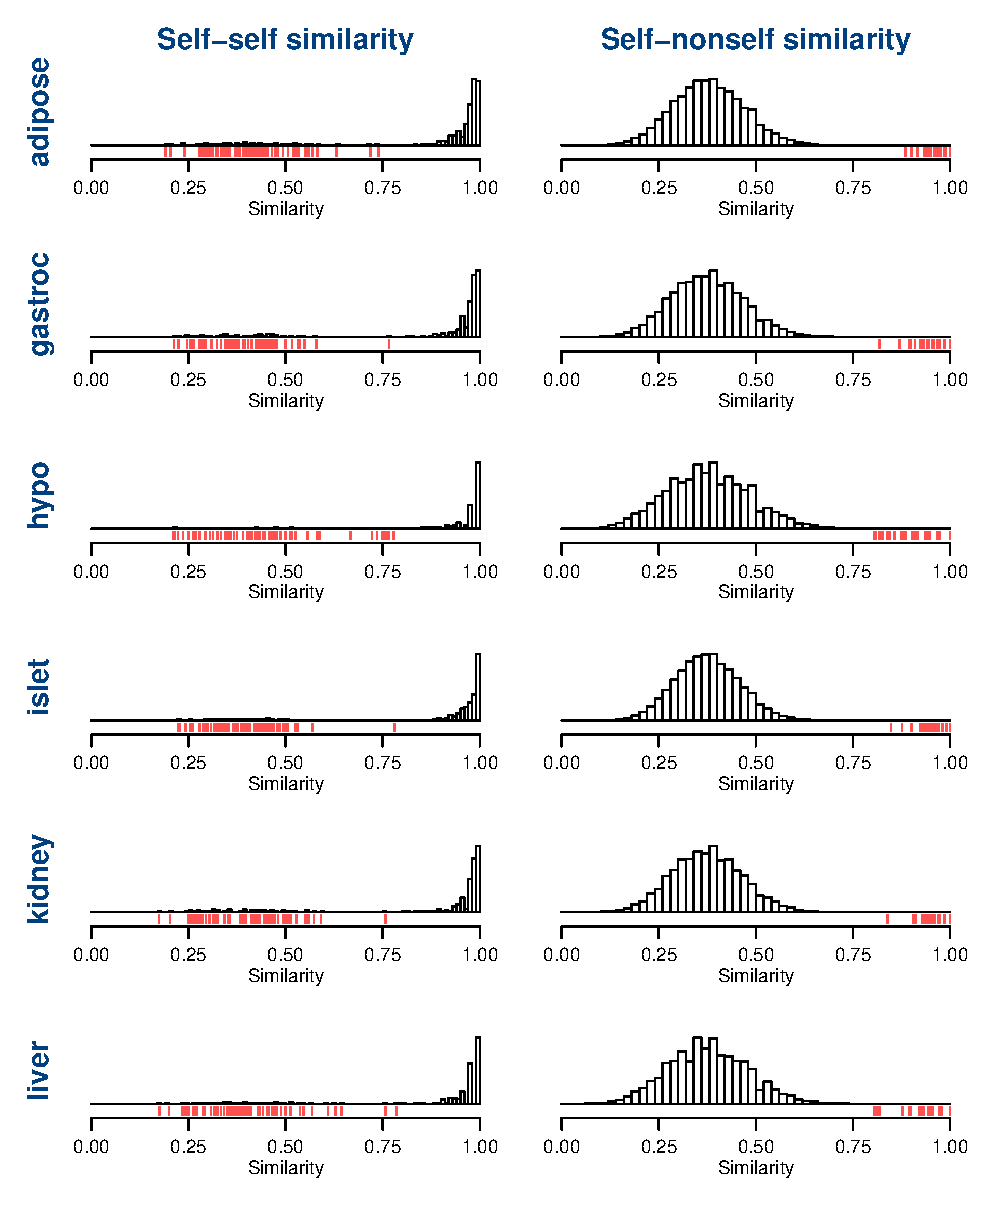
\includegraphics{SuppFigs/figS15.eps}}

\caption{KWB_FIGS15_LEGEND}
\end{figure}



\begin{figure}[p]
\centerline{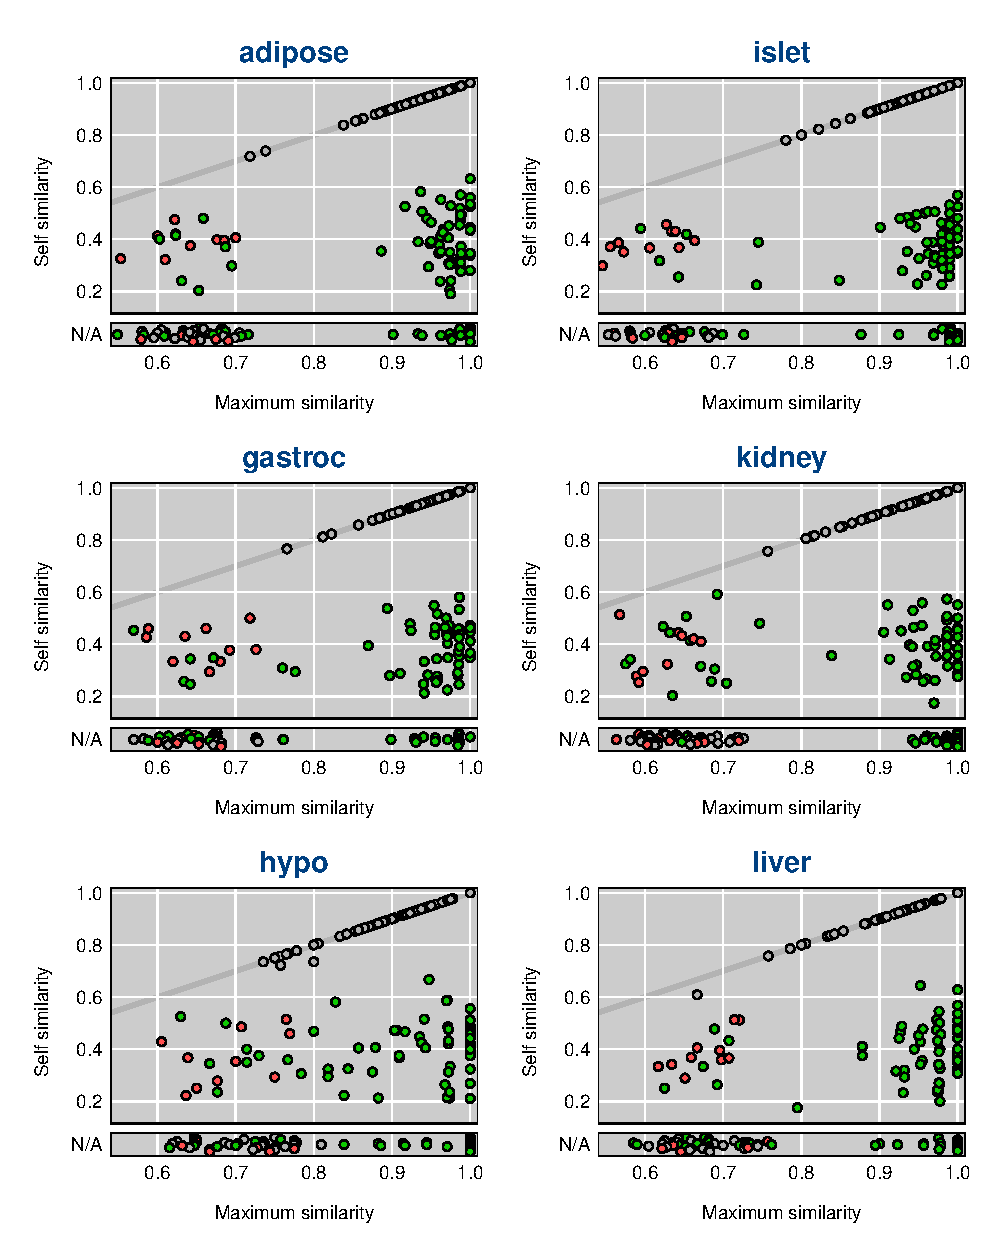
\includegraphics[height=7.65in]{SuppFigs/figS16.eps}}

\caption{KWB_FIGS16_LEGEND}
\end{figure}


\clearpage



\begin{figure}[p]
\centerline{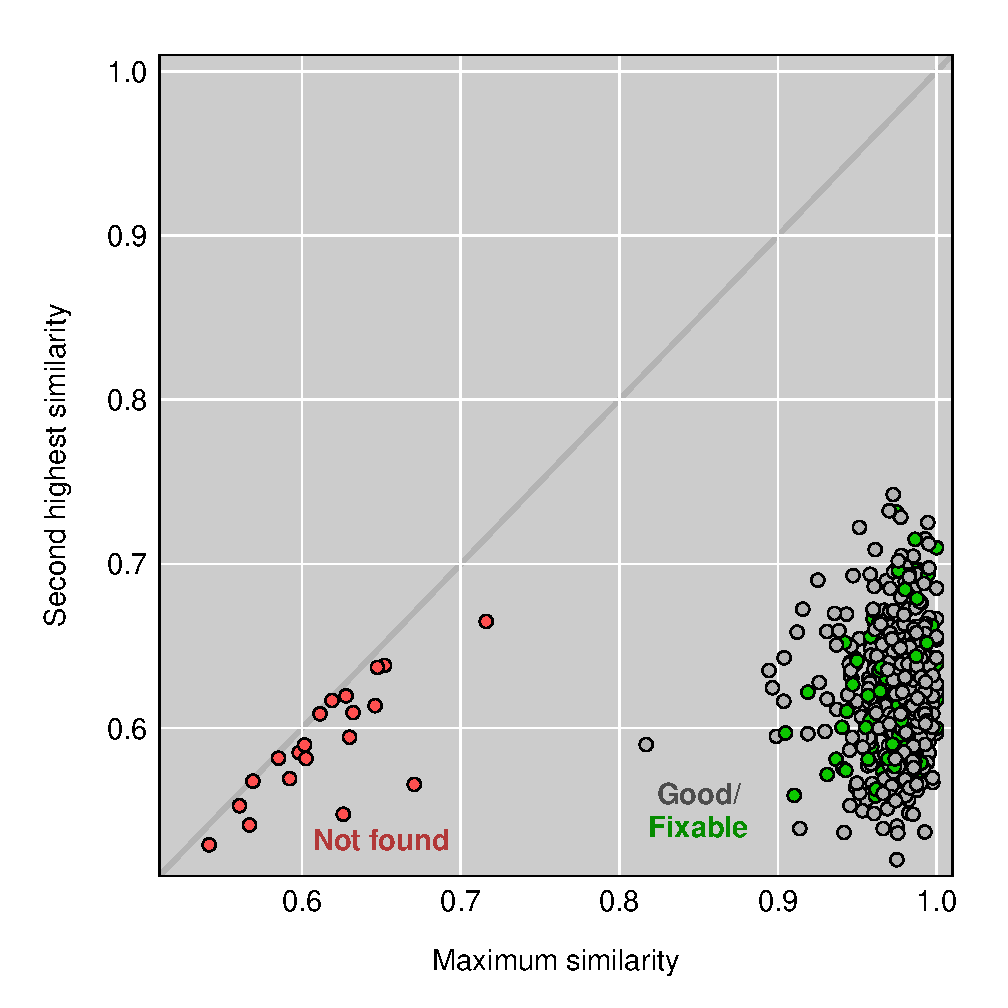
\includegraphics[width=4.5in]{SuppFigs/figS17.eps}}

\caption{KWB_FIGS17_LEGEND}
\end{figure}


\clearpage




\begin{figure}[p]
\centerline{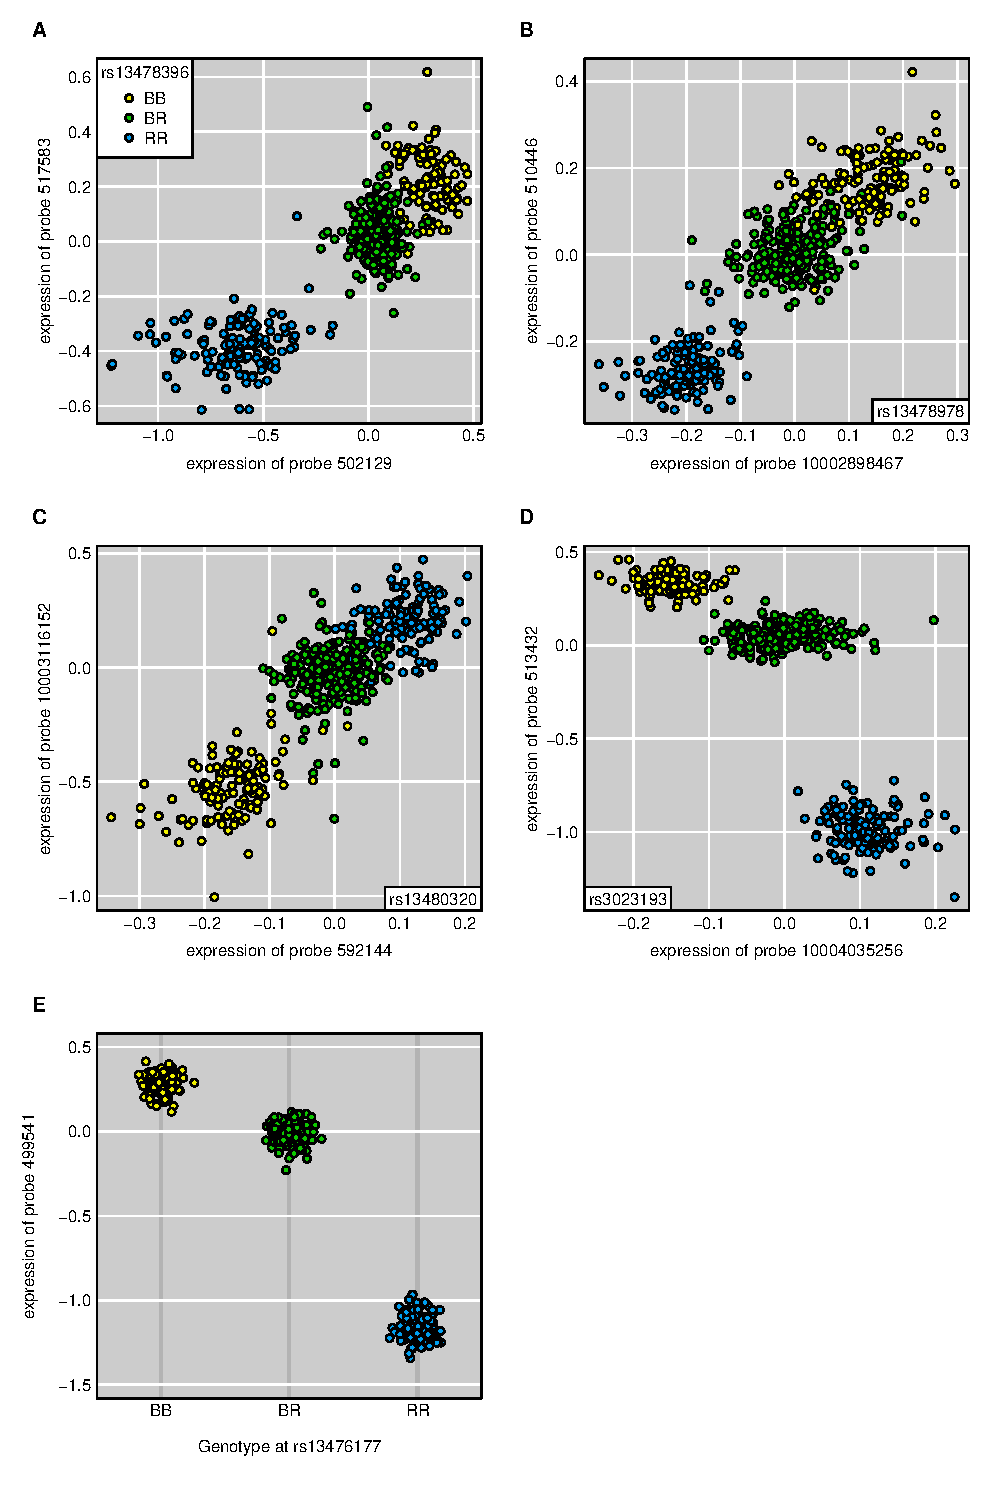
\includegraphics[width=0.85\textwidth]{SuppFigs/figS18.eps}}

\caption{KWB_FIGS18_LEGEND}
\end{figure}

\clearpage




\begin{figure}[p]
\centerline{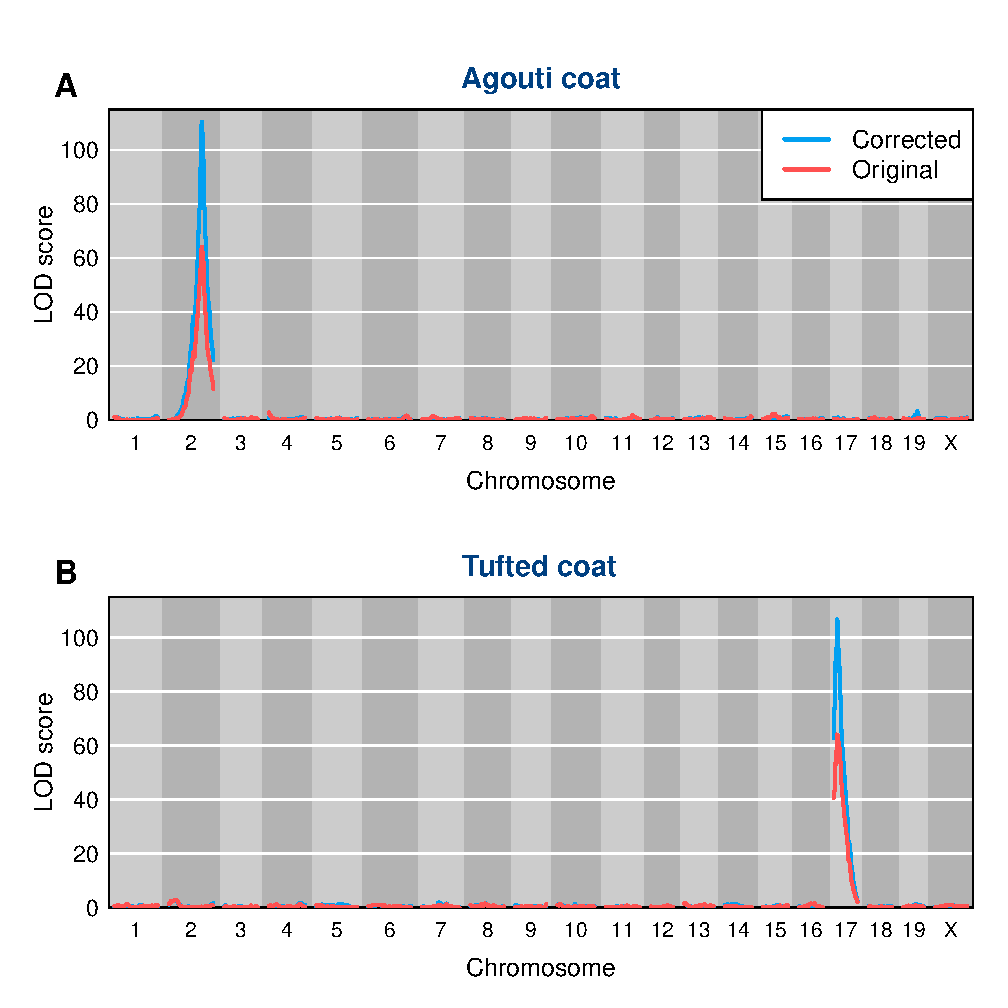
\includegraphics{SuppFigs/figS19.eps}}

\caption{KWB_FIGS19_LEGEND}
\end{figure}




\begin{figure}[p]
\centerline{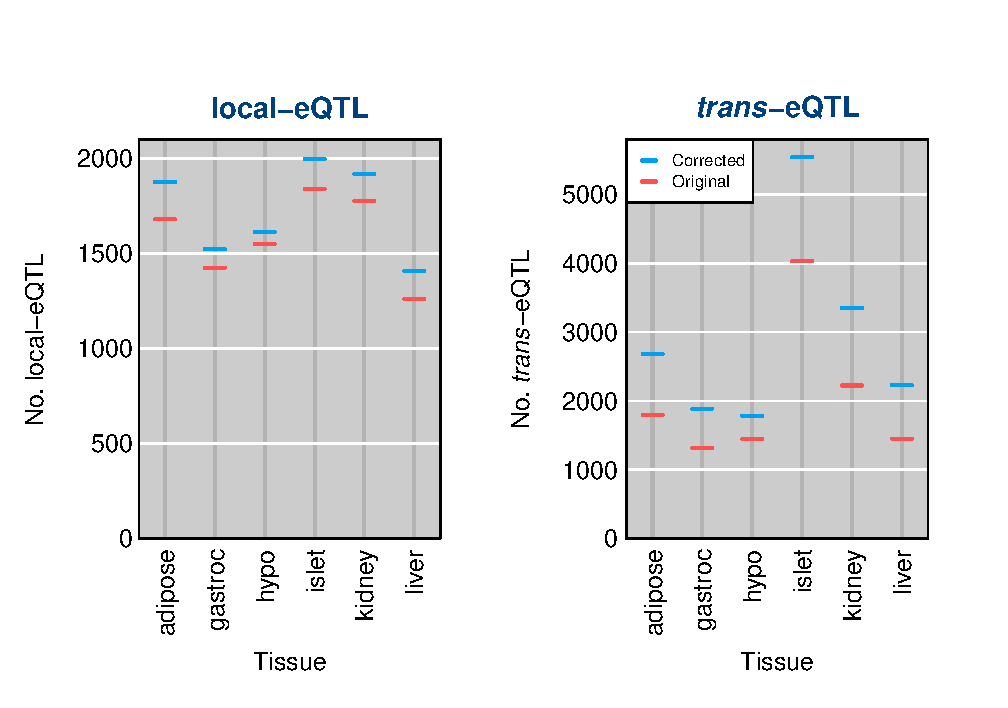
\includegraphics{SuppFigs/figS20.eps}}

\caption{KWB_FIGS20_LEGEND}
\end{figure}




\clearpage

\renewcommand{\arraystretch}{1.5}
\input{SuppTables/tableS1.tex}

\clearpage

\input{SuppTables/tableS2.tex}

\clearpage

\input{SuppTables/tableS3.tex}

\clearpage

\input{SuppTables/tableS4.tex}

\clearpage

\input{SuppTables/tableS5.tex}

\end{document}
